\documentclass[a4paper,10pt]{article}
%\documentclass[a4paper,10pt]{scrartcl}

\usepackage[utf8]{inputenc}
\usepackage{graphicx}
\usepackage{float}
\usepackage{anysize}

\marginsize{2cm}{2cm}{1cm}{1cm}
\title{Documentación de los programas, tarea 1 elo329.}
\author{Pascal Ernesto Sigel Olivares}
\date{abril-2014}

\pdfinfo{%
  /Title    (Documentación tarea 1 de Programación orientada a objetos UTFSM, 2014 Semestre 1)
  /Author   (Pascal Ernesto Sigel Olivares)
  /Creator  (Pascal Ernesto Sigel Olivares)
  /Producer ()
  /Subject  ()
  /Keywords (Programación orientada a objetos, POO, UTFSM, elo329, Simulación de experimentos simples, simulación)
}

\begin{document}
\maketitle
\newpage
\section{Introducción:}


En el presente documento se explicará cada uno de los programas los cuales están cada uno en su carpeta personal llamada etapa(n) donde n 
es un número. El proyecto está separado en varias etapas, desde la número 1 hasta la número 5 y cada etapa agrega alguna característica a 
la anterior.\newline

El proyecto en sí es un simulador de interacciones físicas como, por ejemplo, el choque de dos bolas, una bola junto con un resorte 
o un bloque con rose con bolas y resortes en cualquier disposición deseada.\newline

En la próxima sección se mostrarán algunos detalles importantes de el programa etapa1, que consta de dos bolas una en resposo y la otra en 
movimiento que chocan con choque elástico.

\section{Etapa 1}

El programa etapa 1 es la primera versión de este simulador el cual simula la interacción de dos bolas que chocan. 
En este programa se crea la primera versión del simulador con las clases PhysicsLab,MyWorld, PhysicsElement y Ball. Se hará
una descripción de cada una de estas clases.\newline

\subsection{Clase PhysicsLab:}


La clase PhysicsLab es la clase main del proyecto, esta clase manipula el objeto de tipo MyWorld creándolo y dándole los elementos que
interaccionarán en este ``mundo'' simulado.\newline

\subsection{Clase MyWorld:}


Esta clase es la que maneja la interacción entre los elementos del mundo simulado, el método principal de esta clase es el método \textbf{simulate}
el cual comienza la simulación. En la función \textbf{simulate} 
se requiere que cada elemento físico (PhysycsElement) sea capaz de calcular su próximo estado.\newline

\subsection{PhysicsElement:}


Los elementos físicos son una clase abstracta de la cual nacen los elementos como bolas, resores, bloques y cualquier otro elemento físico.\newline

\subsection{Ball:}


Esta clase se extiende (desciende) de la clase PhysicsElement y representa una bola la cual tiene masa, velocidad y posicion. En esta clase 
se calcula el próximo estado.\newline


\subsection{Experimento y resultados:}

Lease el archivo README para ejecutar el programa.\newline

El caso ha simular puede ser representado con la siguiente figura:

\begin{figure}[H]
 \centering
 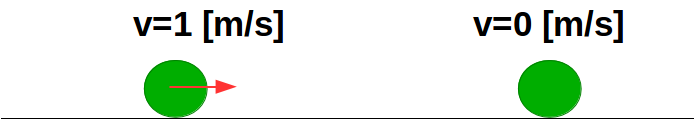
\includegraphics[scale=0.3]{./FigureA.png}
 \caption{Simulación realizada en etapa 1, en la simulación la posición de la bola con velocidad es x=1[mts] y la otra es en x=2.56[mts] ambos con radio 0.1 [mts].}
  \label{etapa1.1}
\end{figure}


Se ha simulado la situación descrita en la figura \ref{etapa1.1}, o sea el choque elástico entre dos
bolas, con la simulación se obtuvieron el siguiente gráfico.

\begin{figure}[H]
 \centering
 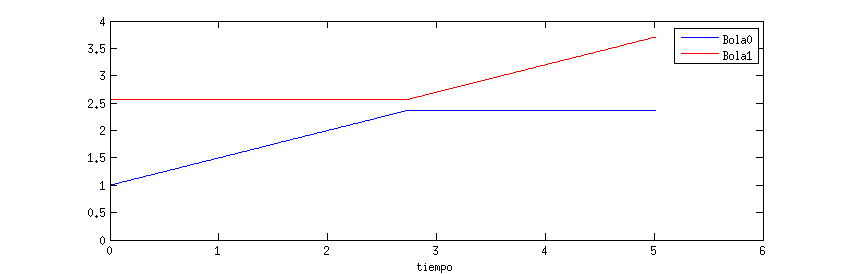
\includegraphics[scale=0.5]{./simulacion_etapa1.png}
 \caption{Resultados simulación etapa 1, Bola 0: bola inicialmente en movimiento y Bola 1: vola inicialmente en reposo.}
  \label{etapa1.2}
\end{figure}

Como se observa en el gráfico de la figura \ref{etapa1.2} cuando la bola 0 colisiona con la bola 1 (a 0.2 mts de distancia dado sus radios) 
la bola 1 obtiene todo el movimiento como se esperaría de un choque elástico de dos masas iguales y una en reposo.\newline

\subsection{Problemas que ocurrieron:}
\subsubsection{Problema con formatos:}
Por defecto Java usa el formato de numeros flotantes con coma ``,'' pero software como matlab usan el formato flotante con punto ``.''
Por lo que en vez de usar \textbf{System.out.print()} se usó \textbf{System.out.format(Locale.US, ... )}.\newline

\end{document}